\documentclass{article}

\usepackage{graphicx}
\usepackage{fullpage}
\usepackage{listings}
\usepackage{url}
\usepackage{amsmath}

\title{Introduction to Python (v2.7) and Programming}
\author{Patrick Steele}
\date{\today}

\lstset{%
  showstringspaces=false,
  numbers=left,
  frame=single,
  language=python
}

\newcommand{\example}[1]{%
  \par
  \vspace{.5em}
  \noindent \texttt{Source of #1}
  \lstinputlisting{../examples/#1}
  \vspace{.5em}
}

\newcommand{\exampleoutput}[1]{%
  \par
  \vspace{.5em}
  \lstinputlisting[frame=single]{../results/#1}
  \vspace{.5em}
}

\begin{document}

\maketitle

\tableofcontents

\section{Introduction}

This guide is intended to a project-based introduction to programming
using Python as our language of choice. This is not intended to be a
Python tutorial, although you will certainly learn some Python along
the way; rather, you should use this guide as a source of problems to
solve (and for some helpful hints for solving them) alongside a
reference such as \url{diveintopython.net} or
\url{http://docs.python.org/2/tutorial/}. This is, perhaps, not
entirely suitable for a \textit{first} introduction to programming,
but is certainly not directed at even moderately advanced programmers.

\subsection{Getting the materials}

This project is hosted at github.com; if you have Git, feel free to
\begin{lstlisting}[language=bash]
> git clone git://github.com/patrickrsteele/learn-python.git
\end{lstlisting}
and get cracking. Otherwise, you can download a zipped copy of the
guide at
\url{raw.github.com/patrickrsteele/learn-python/guide.zip}. Extract
the archive somewhere, which will contain the \texttt{learn-python}
directory.

\subsection{Using this guide}

Throughout this document we will refer to example code; this is
located in the \texttt{examples} directory. For example, to run the
example \texttt{hello.py}, you would run the commands
\begin{lstlisting}[language=bash]
cd path-to-this-directory/src
python hello.py
\end{lstlisting}
in your terminal. To make our notation easier, from here on out we
assume that this guide is located at \texttt{\~{}/learn-python}, and
so to run the \texttt{hello.py} we would run the commands
\begin{lstlisting}[language=bash]
cd ~/guide/src
python hello.py
\end{lstlisting}
Often when referring to an example we will not include the code in the
guide because the code is lengthy; however, we will sometimes include
a small portion of the code. For example, here is the complete source
code of \texttt{hello.py}:
\example{hello.py}
The output of \texttt{hello.py} is
\exampleoutput{hello.out}
All examples are designed for Python~2.7; however, aside from minor
syntax issues, most code should more or less be immediately portable
to Python~3. In particular, we use \texttt{print(s)} syntax rather
than \texttt{print s} syntax.

\subsection{Organization}

This first section offers a brief overview of the
guide. Section~\ref{sec:syntax} offers a \textit{brief} overview of
the syntax of Python. This guide is \textbf{not} meant to be a
reference on the language; rather, this guide is meant to offer
interesting exercises to help you learn Python, and more generally is
meant to be a brief introduction to programming in
general. Section~\ref{sec:flow} introduces the concept of looping and
branching in a program. Later sections offer an overview of challenge
projects. Each challenge project lives in a subdirectory of
\texttt{~/guide/projects}, and comes with a suite tests to validate
your work; feel free to look at the testing code! All the information
needed to complete the projects will be in the source files, but this
document will offer an overview of the project and some helpful design
hints.

\subsection{Object oriented programming}

This guide is not an introduction to object oriented programming
(OOP); feel free to use OOP principles in your solutions, but I am not
going to talk about classes, inheritance, or any other OOP
buzzwords. Other books do a far better job than I will explaining
these principles, and you can go \textit{very} far in Python without
needing classes.

\section{Python syntax}
\label{sec:syntax}

Python programs are contained in text files ended with the file
extension \texttt{.py}. The files contain a number of declarations and
expressions; declarations describe data and behavior, while
expressions perform some action. Generally each line of the file makes
a single declaration or executes a single expression, but this is not
a rule. Whitespace (spaces, tabs, and newlines) is significant in
Python. Instead of using paired curly braces to denote blocks of code
as in C or Java, Python uses indentation; for this reason, your Python
code should uniformly use either tabs or spaces for indentation, and
you cannot arbitrarily indent lines. In general, a line of code must
have the same amount of indentation as the previous line, unless the
new line enters or leaves a new block of code. For example, consider a
simple program that decides if a user-provided number is positive or
non-positive:
\example{positive.py}
If you run this program and provide the number 7 as input, the output
will be
\exampleoutput{positive-pos.out}
while if you enter -7, the output will be
\exampleoutput{positive-neg.out}
Note that the code that depends on the sign of the input is
indented. This means that line~3 is the block of code executed when
line~2 has a true value, while line 5 is the block of code
executed when line~2 has a false value. In either case, line 6 share
the same level of indentation as lines~1,~2, and~4, and so is executed
no matter which indented block is executed; when the indented blocks
are finished, we move one level of indentation \textit{left} to
continue execution.

\section{Program flow}
\label{sec:flow}

As a Python program executes, it follows a series of instructions to
know what to do. Unless we tell it otherwise, the program executes
line-by-line, in order. This isn't always what we want, as we
sometimes want our program to do different things based on data. For
example, consider the behavior of a web browser's address bar. If the
user enters a valid url, such as ``www.recipes.com'', we might expect
the browser to visit that site, but if they enter an invalid url, such
as ``how to make a pie'', perhaps we perform a search using Google for
``how to make a pie.'' In this case, we want our program to skip to a
different section of the program and resume execution there. Other
times we wish to repeat behavior some number of times. For example,
consider the address bar again. We don't want it to visit a url or
perform a search after each keystroke; rather, we want it to do
nothing until the enter key is pressed (or the ``go'' button is
clicked''). In this case, we wish for the same section of our program
to be executed over and over again, possibly with different data each
time. These two concepts, branching and looping, are expressed in
Python using \texttt{if}-statements (branching) and \texttt{for}- and
\texttt{while}-loops (looping).

\subsection{Branching: \texttt{if}-statements}

In Python, \texttt{if}-statements are used to choose between several
possible execution paths in a program. At a high level, they capture
the following behavior: ``If $A$ is true, then execute code $B$,
otherwise execute code $C$.'' Specifically, we have some
\textit{predicate} $A$ that evaluates to \texttt{True} or
\texttt{False}, such as \texttt{x < 10} or \texttt{name == "Patrick"},
and we want the behavior of the program to depend on the value of the
predicate. If the predicate is true, we want some code $B$ to be
executed, while if the predicate is false we want some other code $C$
to be executed. Recall the program \texttt{positive.py}:
\example{positive.py}
Here, the predicate $A$is line~2, \texttt{number > 0}. When $A$ is
true, i.e. the variable \texttt{number} stores a value greater than
zero, we execute block $B$, which is line~3, or \texttt{print("You
  entered a positive number")}. When $A$ is false, i.e. the variable
\texttt{number} stores a value that is less than or equal to zero, we
execute block $C$, which is line~5, or \texttt{print("You entered a
  non-positive number")}. In either case, whether $A$ is true or
false, we go on to execute line~6, \texttt{print("Exiting program")},
since only lines~2 through~5 are involved in the
\texttt{if}-statement; we can see this because blocks $B$ and $C$ are
indented one more level than the first line, the predicate line $A$,
and the final line~6. See figure~\ref{fig:positive} for a schematic
diagram of the flow of execution in the program \texttt{positive.py}.

\begin{figure}[htp]
  \centering
  
  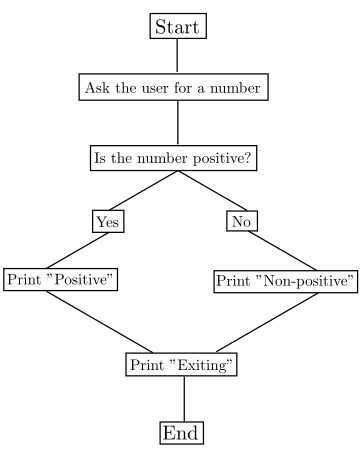
\includegraphics[width=3in]{img/if-statement.eps}

  \caption{A schematic of the flow of the program
    \texttt{positive.py}.}
  \label{fig:positive}
\end{figure}

\subsection{Looping: \texttt{while}-loops}

\texttt{while}-loops are one looping construct used in Python. At a
high level, they capture the following behavior: ``While $A$ is true,
execute some code $B$.'' Again, $A$ is a predicate that evaluates to
\texttt{True} or \texttt{False}, and $B$ is a block of code to be
evaluated each time predicate $A$ is found to be true. Note that block
$B$ most likely affects some values involved in $A$, or else $A$ would
remain true forever.

To illustrate the \texttt{while}-loop, we create a program that prints
out the integers $1$, $2$, $\ldots$, $10$. The code is
\example{while.py}
and has output
\exampleoutput{while.out}
Here the predicate is line~2, \texttt{n <= 10}, while the block $B$
are lines~3 and~4, \texttt{print(n)} and \texttt{n = n + 1}. Note that
line~5 is executed no matter how many times $B$ is executed. A
schematic diagram of the flow of execution of the program is shown in figure~\ref{fig:while-loop}.

\begin{figure}[htp]
  \centering
  
  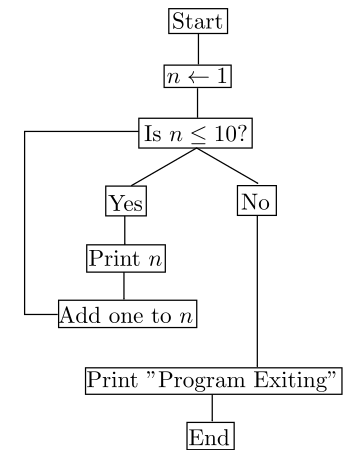
\includegraphics[width=3in]{img/while-loop.eps}

  \caption{A schematic of the flow of the program
    \texttt{while.py}.}
  \label{fig:while-loop}
\end{figure}

\subsection{Looping: \texttt{for}-loops}

A \texttt{for}-loop is really just special syntax for quickly listing
all the items in a collection. Consider an array of integers
\texttt{a}, say \texttt{a = [1, 3, 5, 7, 9]}. We might want to print
out the square of each number in the list; using a while loop, we
might write the following code
\example{for-while.py}
which produces the output
\exampleoutput{for-while.out}
However, we often find ourselves trying to do something to each
element of a list, and so we have the \texttt{for}-loop. We could
re-write the previous program as
\example{for-for.py}
which has the same output
\exampleoutput{for-for.out}
This code is substantially simpler in that we do not need to track the
index variable \texttt{n}; in general, whenever you are not interested
in the location of the data in a collection, but only the data itself,
you can use a \texttt{for}-loop.

At a high level, \texttt{for}-loops capture the following behavior:
for each element $X$ in a collection $C$, execute a block of code
$B$. Note that the code in $B$ will have access to the current value
of variable $X$. It is important to understand that a
\texttt{for}-loop offers nothing fundamentally more than the
\texttt{while}-loop; you can re-write any program that uses
\texttt{for}-loops to instead use \texttt{while}-loops without
changing the behavior of the program. For this reason,
\texttt{for}-loops can be thought of as \textit{syntactic sugar}, as
they greatly improve the expressiveness of the language and allow for
ideas to be expressed in fewer lines of code, but are completely
unnecessary to write correct programs. Do not, however, let this
dissuade you from using \texttt{for}-loops in your code; in fact,
idiomatic Python code generally uses \texttt{for}-loops over
\texttt{while}-loops whenever possible.

\subsubsection{A note for Java and C programmers}

There is no analogue of Java- or C-style \texttt{for (\textit{init},
  \textit{cond}, \textit{increment}) \{...\}} for loops in Python. Use
a \texttt{while}-loop instead if you really want this behavior.

\subsection{Flow control: Test}

We will now try to write a program that utilizes both the
\texttt{while}-loop and \texttt{if}-statement. Try to write a program
that implements the program diagrammed in
figure~\ref{fig:flow-test}. The output of the program should be
\exampleoutput{flow-test-bad.out}
Note that you could create this output with a program like
\example{flow-test-bad.py}
but this program does not generalize for different sized loops.

\begin{figure}[htp]
  \centering
  
  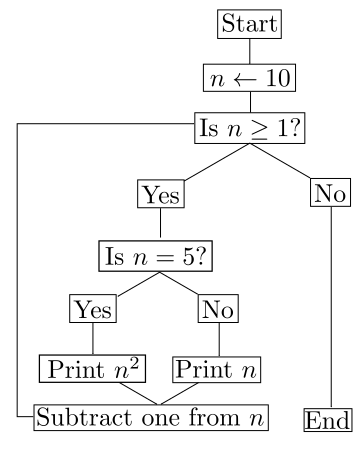
\includegraphics[width=3in]{img/flow-test.eps}

  \caption{A schematic of the flow of a program that should utilize
    both a \texttt{while}-loop and \texttt{if}-statement.}
  \label{fig:flow-test}
\end{figure}

\section{Project: Functions}

This first project is designed to get you familiar with functions in
Python. Broadly, a function is a piece of code that accepts some
inputs and produces some outputs. This code can be re-used with
different inputs many times throughout a program. For example, you
might want to calculate the sales tax at many different places in your
program. You could simply write \texttt{x * .05} to compute a
5\%~sales tax on the quantity \texttt{x}, but if the rate changes
you're going to have to hunt through your code to find each time you
computed the sales tax. A better idea would be to define a function
\texttt{tax} that takes as input a single number, and returns the tax
associated with it. For example, we can compute a 5\%-sales tax on
\$100, \$200, and \$300 using the program
\example{tax.py}
which has output
\exampleoutput{tax.out}
Functions do not need to have input or output; for example, the
function \texttt{greeting} defined in as
\example{greeting.py}
does not take any input arguments, and does not return a
value. However, this function produces a \textit{side effect} of
printing out text. The output is below.
\exampleoutput{greeting.out}
Note that we referred to printing a value as a side effect; this is
because it would be difficult (but not impossible) for the program to
know that \textit{greeting} printed out a value; if the program needs
to know what was printed, we should rather define a function like
\example{greeting-return.py}
which produces identical output:
\exampleoutput{greeting-return.out}

We now introduce our first programming project. In the
\texttt{\~{}/guide/project/functions} directory there is are files
\texttt{functions-1.py} and \texttt{test.py}. \texttt{functions-1.py}
contains the stubs of functions that you should complete; the comments
in each function tell you how the function should behave. When you
think your functions are correct, you can test your work by running
\texttt{python test.py}, which will run tests against your code. The
first several lines of output of these tests should look like

\vspace{.5em}
\lstinputlisting[frame=single,lastline=20]{../results/functions-test.out}
\hfill \textit{$\vdots\qquad$ some content omitted... $\qquad\vdots$} \hfill
\vspace{.5em}
\lstinputlisting[frame=single,firstline=75]{../results/functions-test.out}

\noindent As you can see, the output of the tests are broken into
distinct \textit{test cases}, each corresponding to a test
function. For example, on line~6, we see that there was a failure in
function the test function \texttt{test\_mean\_1}, which tests that
the mean of an empty list is zero. Since we have yet to correctly
define the \texttt{mean} function in \texttt{functions-1.py}, this
test of course fails. The first line of the output is a series of
``F'' and ``.''  characters; each ``F'' corresponds to a failed test,
while each ``.''  character corresponds to a passed test. The final
three lines tell us that~7 tests were run in total, and all~7 failed.

\section{Project: Data structures}

This project is designed to introduce more advanced usage of Python
lists and dictionaries as building blocks for more complex data
structures.

Data structures in computer programming are a way of representing
structured data in a way that makes it easy to manipulate. For
example, consider making an attendance program. We want to be able to
store a list of people that have showed up to a meeting, and for each
person store their first name, last name, and company ID number. In
particular, suppose that ``Smith, John (id 1),'' ``Smith, Jane (id
7)'' and ``Miller, Sally (id 20)'' show up. We
could simply use a list of lists, and store this data as
\begin{lstlisting}
[["Smith", "John", 1], ["Smith", "Jane", 7], ["Miller", "Sally", 20]]
\end{lstlisting}
However, such data could be difficult to work with. If you want a last
name, you have to remember that it is being stored in index~0, while
first names are stored in index~1, and company IDs are stored in
index~2. However, the indices we store the data in have no relation to
the data, and so we would like to avoid using indices at all. Perhaps
a better way to store this information would be to have a list of
dictionaries:
\begin{lstlisting}
  [{"last": "Smith", "first": "John", "id": 1},
   {"last": "Smith", "first": "Jane", "id": 7},
   {"last": "Miller", "first": "Sally", "id": 20}]
\end{lstlisting}

\section{Project: Project Euler}

This last project isn't my work at all, but is a great next step. Go
to \url{projecteuler.net}, sign up, and start solving problems! From
\url{projecteuler.net}, 
\begin{quote}
  \hspace{-.85em} ``Project Euler is a series of challenging
  mathematical/computer programming problems that will require more
  than just mathematical insights to solve. Although mathematics will
  help you arrive at elegant and efficient methods, the use of a
  computer and programming skills will be required to solve most
  problems.''
\end{quote}
Unlike project up to this point, Project Euler doesn't validate your
code directly; rather, they formulate a problem and an input, and then
have a text box where you can enter your solution. If your solution is
correct, you are granted access to the discussion forum for that
problem where you can see how others solved the problem, and if you
get it wrong, you get to try again. The first problem on the site is
stated as:
\begin{quote}
  If we list all the natural numbers below 10 that are multiples of 3
  or 5, we get 3, 5, 6 and 9. The sum of these multiples is 23.

  Find the sum of all the multiples of 3 or 5 below 1000.
\end{quote}
The problems often follow the pattern of providing a simple input and
the correct solution corresponding to it, and then asking you to solve
the same problem on more difficult inputs. The problems grow in
difficultly (although not strictly) as you progress (and you may
progress in any order; if you get stuck, move on!). For example,
problem~50 is stated as:
\begin{quote}
  The prime 41, can be written as the sum of six consecutive primes:
  \begin{equation*}
    41 = 2 + 3 + 5 + 7 + 11 + 13
  \end{equation*}
  This is the longest sum of consecutive primes that adds to a prime
  below one-hundred.

  The longest sum of consecutive primes below one-thousand that adds
  to a prime, contains 21 terms, and is equal to 953.

  Which prime, below one-million, can be written as the sum of the
  most consecutive primes?
\end{quote}

\end{document}
%  LocalWords:  Whitespace subdirectory OOP indices
